\documentclass[12pt,a4paper]{report}
\usepackage[brazil]{babel}
\usepackage[]{algorithm}
\usepackage[]{algorithmic}

\usepackage[style=numeric,backend=biber]{biblatex}
\usepackage[utf8]{inputenc}
\usepackage{kpfonts}
\usepackage[T1]{fontenc}
\usepackage{wrapfig}
\usepackage{graphicx}
\usepackage{enumerate}
\usepackage{subcaption}
\usepackage{float}
\usepackage{caption}
\usepackage{listings}
\usepackage{lipsum}
\usepackage{amsthm}
\usepackage{amssymb}
\usepackage{bm}
\usepackage{color}
\usepackage{afterpage}
\usepackage[inline]{enumitem}
\usepackage{pdflscape}
\usepackage{listingsutf8}
\usepackage{siunitx}
\usepackage{bashful}

\usepackage[margin=1in]{geometry}

\lstset{frame=tb,
  aboveskip=2mm,
  belowskip=2mm,
  showstringspaces=false,
  columns=flexible,
  basicstyle=\footnotesize,,
  numbers=left,
  numbersep=5pt,
  stepnumber=1,
  breaklines=true,
  keepspaces=true,
  breakatwhitespace=true,
  showtabs=false,  
  tabsize=2
}


% Definindo estilo para os códigos
\definecolor{mGreen}{rgb}{0,0.6,0}
\definecolor{mGray}{rgb}{0.5,0.5,0.5}
\definecolor{mPurple}{rgb}{0.58,0,0.82}
\definecolor{dkgreen}{rgb}{0,0.6,0}
\definecolor{backgroundColour}{rgb}{0.97,0.97,0.97}

\lstset{basicstyle=\ttfamily,
    backgroundcolor=\color{backgroundColour},   
    commentstyle=\color{mGreen},
    keywordstyle=\color{magenta},
    numberstyle=\tiny\color{mGray},
    commentstyle=\color{dkgreen},
    stringstyle=\color{mPurple},
    basicstyle=\footnotesize,
    breakatwhitespace=false\textbf{,}         
    breaklines=true,                 
    captionpos=b,                    
    keepspaces=true,                 
    numbers=left,                    
    numbersep=5pt,                  
    showspaces=false,                
    showstringspaces=false,
    showtabs=false,                  
    tabsize=2,
    language=bash
}

\lstdefinestyle{BStyle}{
    backgroundcolor=\color{backgroundColour},  
    showstringspaces=false,
    numbers=none,
    language=bash
}

\pagenumbering{arabic}
\renewcommand{\thesection}{\arabic{section}}

\bibliography{ref}
\renewcommand{\contentsname}{Sumário}{\thispagestyle{empty}}
\renewcommand{\baselinestretch}{1.5} 

\begin{document}

\begin{titlepage}
        \begin{center}
                \vspace*{1cm}
                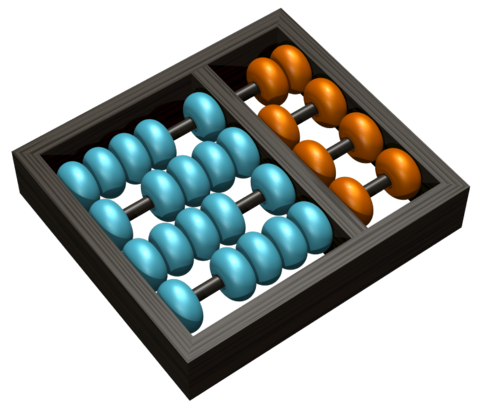
\includegraphics[width=0.25\textwidth]{Logo}\\
                \vspace{1.5cm}
                \Huge
                \textbf{Exercício 2.2}\\
                \vspace{1.5cm}
                \Large
                \textbf{Aluno}: João Vitor Gonçalves\\
                \textbf{RA}: 176353\\
                \vspace{1.2cm}
                \Large
                Instituto de Computação\\
                Universidade Estadual de Campinas\\
                \vspace{1.5cm}
                Campinas, 30 de Outubro de 2020.
        \end{center}
\end{titlepage}
\tableofcontents
\clearpage

\newcommand{\shellcmd}[1]{\texttt{\footnotesize\# #1}}%estilizando citação de comandos do shell

% \section{Insertion Sort}

% \subsubsection{Pseudocódigo}
% \begin{algorithm}
% \caption{InsertionSort(A)}
% \begin{algorithmic}[1]
%     \STATE $A[0] \longleftarrow -\alpha$
%   \STATE $i \longleftarrow 2 $
%     \FOR {$i$ to $N $} 
%             \STATE $j \longleftarrow i$

%             \WHILE{$A[j] > A[j-1]$} 
%                 \STATE $T \longleftarrow A[j-1]$ 
%                 \STATE $A[j-1] \longleftarrow A[j]$ 
%                 \STATE $A[j] \longleftarrow T$ 
%                 \STATE $j = j -1$
%             \ENDWHILE
%     \ENDFOR
%     \RETURN $A$
%     \end{algorithmic}
% \end{algorithm}



\section{Adicione a função sleep no servidor.c da atividade prática anterior antes do socket ser fechado
close(connfd) de modo que o servidor ''segure'' a conexão do primeiro cliente que se conectar. Com
essa modificação, o servidor aceita a conexão de dois clientes de forma concorrente ? Comprove sua
resposta através de testes.}

Com essa modificação, o servidor ainda não consegue aceitar conexões de dois clientes de forma concorrente, o que é compreensível, uma vez que o tratamento das chamadas de conexão dos clientes é feito num loop em uma única thread.

Então o que ocorre é que o servidor aceita a primeira conexão, realiza o sleep, e somente após o sleep e fechar a primeira conexão, aceita a segunda conexão pendente e responde o cliente.

\begin{figure}[H]
  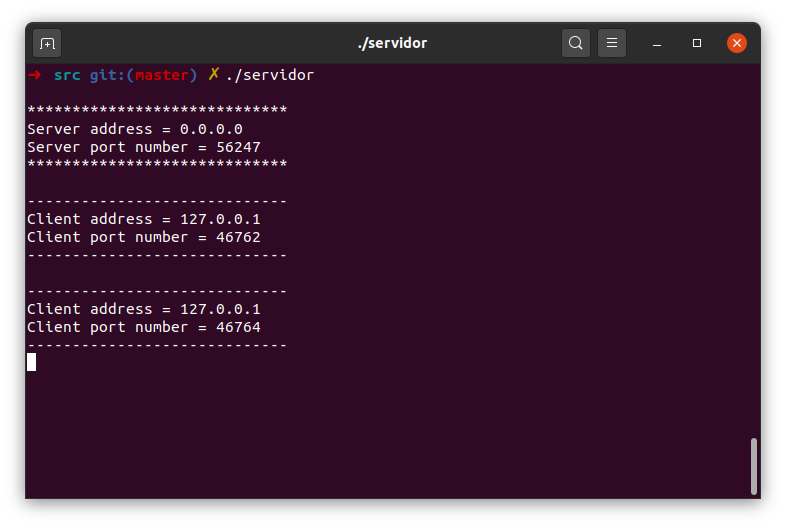
\includegraphics[width=\linewidth]{serv.png}
  \caption{Execução do servidor.}
\end{figure}

\begin{figure}[H]
  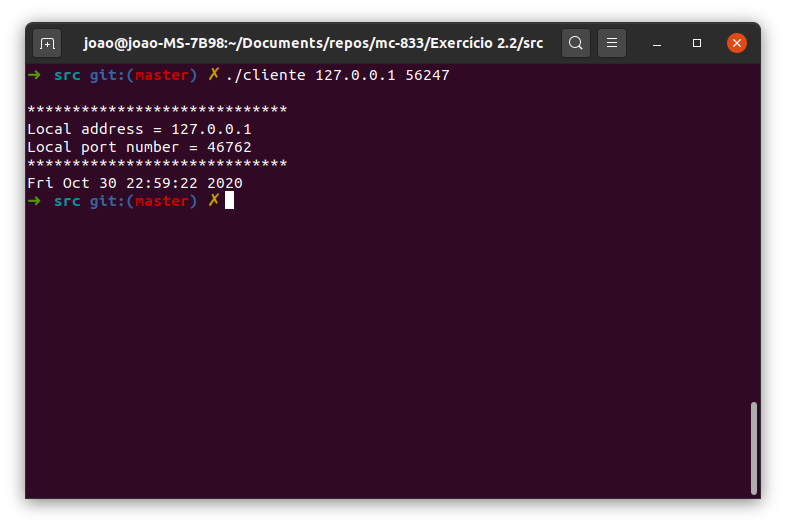
\includegraphics[width=\linewidth]{cliente1.png}
  \caption{Execução do cliente 1.}
\end{figure}

\begin{figure}[H]
  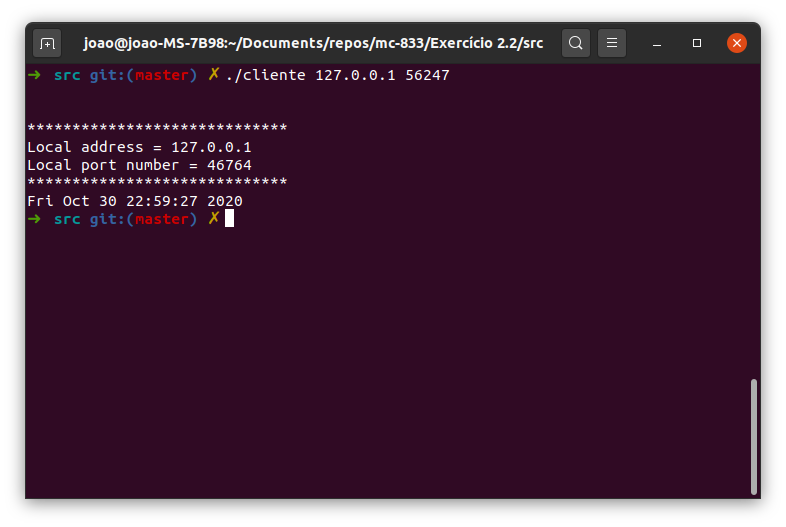
\includegraphics[width=\linewidth]{cliente2.png}
  \caption{Execução do cliente 2.}
\end{figure}

Então como podemos ver pelas imagens. Com um sleep de 5 segundos, o servidor responde o segundo cliente exatamente 5 segundos após o primeiro.

\section{Com base ainda no seu código, é correto afirmar que os clientes nunca receberão FIN neste
caso já que o servidor sempre ficará escutando (LISTEN)? Justifique.}
Sim, é correto. Uma vez que o servidor nunca fecha a conexão com o cliente, e está perpetuamente ouvindo, o \emph{FIN} nunca será enviado.

No caso da implementação particular, isso só não é verdade no caso do cliente enviar uma cadeia de caracteres igual à \emph{exit}, então o servidor irá finalizar a conexão.

\section{Comprove, utilizando ferramentas do sistema operacional, que os processos criados para
manipular cada conexão individual do servidor aos clientes são filhos do processo original que
foi executado.}

O processo pai do servidor foi executado na porta 8585, então espera-se que exista um processo listening na porta 8585.

\begin{figure}[H]
  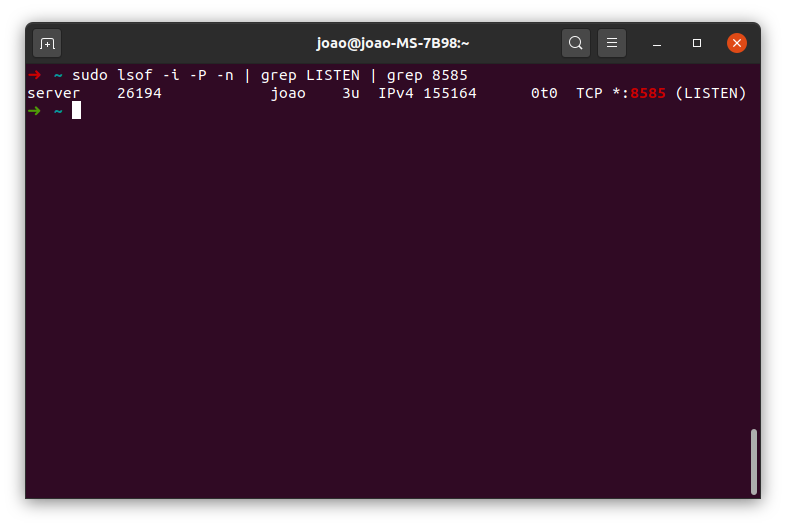
\includegraphics[width=\linewidth]{parent.png}
  \caption{Identificando processo pai.}
\end{figure}

Então usando o comando \emph{lsof} podemos identificar o PID desse processo, que no caso é \textbf{26194}.

Então por meio do compando \emph{ps} conseguimos listar todos os processos filhos desse PID:

\begin{figure}[H]
  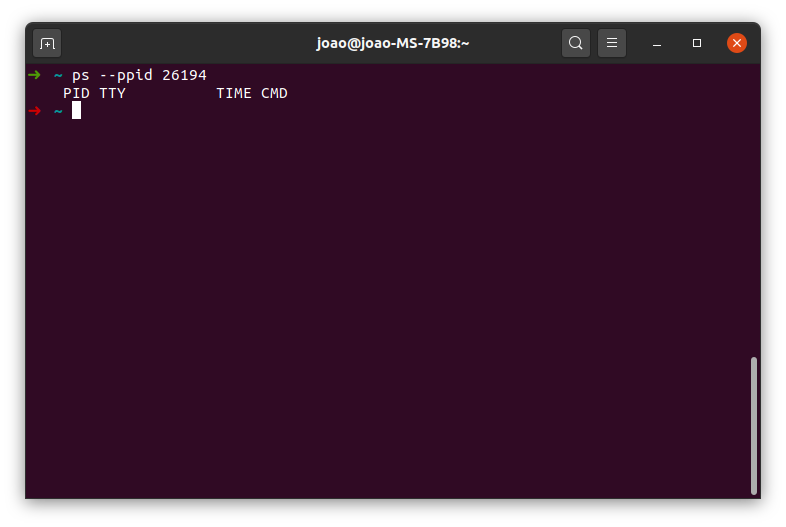
\includegraphics[width=\linewidth]{no_child.png}
  \caption{Identificando processos filhos.}
\end{figure}

Como ainda não temos nenhum cliente sendo executado, essa listagem vem vazia, mas assim que executamos dois filhos em concorrência, observamos:

\begin{figure}[H]
  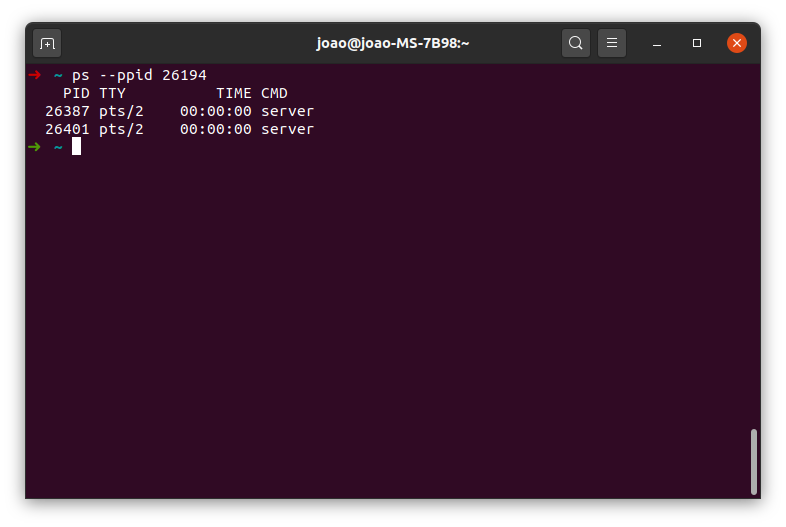
\includegraphics[width=\linewidth]{2_child.png}
  \caption{Identificando processos filhos.}
\end{figure}

E caso a execução de um dos filhos seja interrompida por meio do comando \emph{exit}, temos:

\begin{figure}[H]
  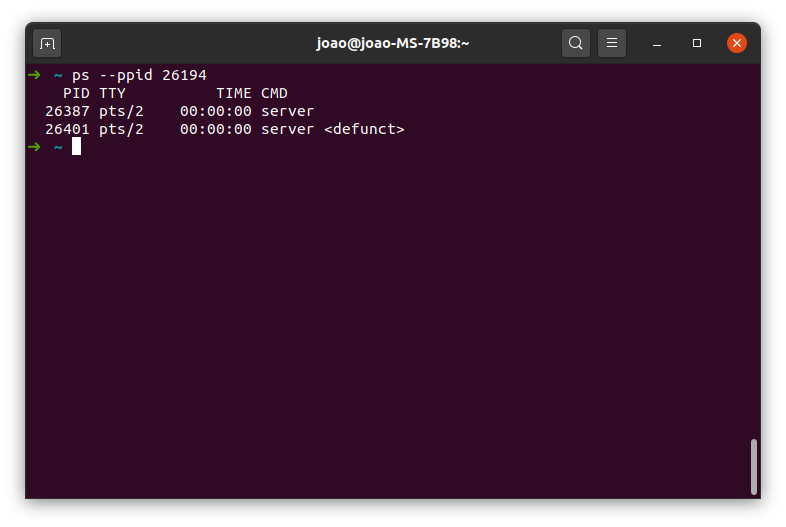
\includegraphics[width=\linewidth]{1_child.png}
  \caption{Identificando processos filhos.}
\end{figure}

Então como podemos observar, o servidor cria novos processos filhos no caso de novas conexões, e os finaliza no caso de desconexão.

\section{Detalhes de implementação}

Esse projeto foi implementado em c++, com o uso da ferramenta \emph{cmake} para simplificar o processo de compilação.

Para compilar o projeto deve ser executado:

\begin{lstlisting}[language=bash]
  cd build
  cmake ..
  make
\end{lstlisting}

O cmake é uma ferramenta utilizada para gerar os MakeFiles de forma automática, pode ser olhado com detalhes que comandos são utilizados para realizar a compilação nos arquivos CMakeLists.txt nas pastas \emph{client/}, \emph{server/} e \emph{socketutils/}.

Como a proposta das funções envelopadoras é para serem reutilizadas em projetos futuros, esses métodos foram externados no projeto \emph{socketutils}, que é importado como biblioteca externa no \emph{server} e \emph{client}.

\subsection{Pastas}
A pasta \emph{lab} contém a implementação em si do exercício, a pasta \emph{ex2} contém a modificação do \emph{sleep} usada no item 1 do trabalho.

\subsection{Execução}

O processo do servidor deve ser executado da seguinte forma:
\begin{lstlisting}[language=bash]
  ./server/server <PORT>
\end{lstlisting}

O processo do cliente deve ser executado da seguinte forma:
\begin{lstlisting}[language=bash]
  ./client/client <SERVER IP> <SERVER PORT>
\end{lstlisting}

\subsection{Comando exit no cliente}
Para que seja possível o cliente capturar o stdin do input, sem bloquear a execução do processo, isso foi feito em uma thread separada da principal. Então à cada execução de um comando do servidor, o cliente irá aguardar 1 segundo por um input do terminal.

Como o cliente escreve o echo na saída padrão, o que está sendo escrito pode acabar se perdendo no meio das linhas sendo printadas, mas se for escrito a cadeia \emph{exit} seguido de um enter, o comando será reconhecido.

\subsection{Arquivos de log}

O servidor irá criar um arquivo para cada conexão aberta para escrever os detalhes. O nome dos arquivos segue o modelo <client-ip>-<client-port>.log

É possível acompanhar a saída de todos os arquivos simultaneamente usando:
\begin{lstlisting}[language=bash]
  tail -F *.log
\end{lstlisting}

Isso foi feito para não termos que lidar com escritas concorrentes dos múltiplos processos.

\subsection{Envio de comandos}

Os comandos serão enviados do servidor para o cliente com um intervalo de 2 segundos para não deixar o stdout do cliente muito rápido.

\end{document}